% v1.1, 2026-08-18: single-thesis revision for research-sample use.
% Governing claim: domain specialization in expert routing is expressed
% during generation and largely absent from prefill; per-domain expert
% winners are concentrated on one generalist over prefill and disperse to
% distinct per-domain experts over generation, in two Qwen3.5 MoE
% checkpoints with unrelated expert indices, and the shift survives a
% token-balanced control. Implication: specialization measured over
% supplied text or pooled across passes is understated; negative results
% from prefill routing are silent about generation; measure the passes
% separately. Changes from v1.0 (June 2026): two-column layout; title;
% "why prefill is tempting" section folded into intro; slogan repetition
% removed; Fig 2 (entropy bars, duplicating Table 1) dropped, 2 figures
% remain; proposed-experiment list removed, limitations kept; audit note
% folded into Data Availability; em-dashes removed; terms defined at
% first use. All v1.0 numeric values retained.
\documentclass[10pt,twocolumn]{article}

\usepackage[letterpaper,margin=0.85in]{geometry}
\usepackage{lmodern}
\usepackage[T1]{fontenc}
\usepackage{microtype}
\usepackage{booktabs}
\usepackage{graphicx}
\usepackage{amsmath}
\usepackage{caption}
\usepackage[round]{natbib}
\usepackage[hidelinks]{hyperref}

\hypersetup{
  pdftitle={Generation-Time Routing Reveals Expert Specialization That Prefill Measurements Miss},
  pdfauthor={Jeffrey Shorthill},
  pdfkeywords={mixture-of-experts, expert specialization, routing, prefill, generation, autoregressive decoding, language models, interpretability, evaluation methodology}
}

\captionsetup{font=small,labelfont=bf}
\setlength{\parskip}{0.2em}
\setlength{\columnsep}{0.28in}

\title{\textbf{Generation-Time Routing Reveals Expert Specialization\\
That Prefill Measurements Miss}}
\author{Jeffrey Shorthill\thanks{Independent researcher. Correspondence:
\texttt{jws299792@icloud.com}. Version~1.1 (August~2026; version~1.0 June~2026),
released under CC~BY~4.0. Concept DOI 10.5281/zenodo.20779604. Data, code, and a
claim-by-claim source index accompany the paper; see Data and Code Availability.}}
\date{}

\begin{document}
\maketitle

\begin{abstract}
In two Qwen3.5 mixture-of-experts (MoE) checkpoints (35B and 122B
parameters) run on 60 prompts spanning twenty academic domains, the expert
that receives the most routing weight in a domain depends on which regime of
the forward pass is measured. Over prefill, when the prompt is processed in
parallel, one generalist expert wins 18 of 20 domains in the smaller model and
13 of 20 in the larger, and routing looks domain-blind. Over generation, when
the answer is produced token by token, the winners disperse to 20 and 18
distinct experts and the generalist wins one or two. The dispersion is a
property of the regime: with prefill and generation matched in token count,
the two regimes select nearly disjoint top-expert sets (Jaccard 0.00 to 0.23)
at unchanged per-token routing entropy (0.958 versus 0.953), so generation
spreads each token over a similar number of experts and routes it to different
ones, and the pattern reproduces across model sizes with unrelated expert
indices. The widely cited negative result that MoE experts do not specialize
by topic was measured over supplied text, which is prefill routing.
Expert-specialization measurements over supplied text, or pooled across
regimes, are therefore understated by construction; prefill-based negative
results are silent about the regime in which specialization is expressed; and
analyses that ask what experts specialize in should separate the two regimes
and read specialization from generation.
\end{abstract}

\section{Introduction}
\label{sec:intro}

Mixture-of-experts (MoE) layers replace a dense feed-forward block with many
parallel expert blocks and a router that selects a few of them for each token.
Because the router makes a discrete, inspectable choice at every token, it
invites a natural question: do the experts divide knowledge by subject? The
most-cited answer is negative. \citet{jiang2024mixtral}, analyzing Mixtral's
routing on validation text, ``do not observe obvious patterns in the assignment
of experts based on the topic''; the structure they find is syntactic and
positional. That result is load-bearing: it is widely read as evidence that MoE
experts do not specialize by domain.

That analysis, and most like it, scored routing over supplied text, and
supplied text is processed in only one of the two regimes in which a
transformer routes tokens. During \emph{prefill}, the whole prompt is processed
in parallel to populate the key/value cache. During \emph{generation}, output
tokens are produced one at a time, each attending to everything before it.
Prefill routing is the natural place to look: it is deterministic given the
prompt and the weights, cheap to capture in a single forward pass, and it is
where the prompt's content sits, so topical routing is intuitively expected to
be strongest there. Routing happens in both regimes, however, and nothing
requires them to agree.

They disagree in a specific, consistent way that decides whether domain
specialization is visible. On a domain-balanced prompt suite run through two
MoE models, the expert that receives the most routing weight in each of
twenty domains is a single generalist for 18 of 20 domains in the smaller
model and 13 of 20 in the larger when routing is read over prefill positions,
and a distinct expert for nearly every domain when the same prompts are read
over generated positions. The dispersion survives a control that matches
prefill and generation in token count, and it reproduces in the larger model
with unrelated expert indices. Prefill routing reproduces the familiar
domain-blind picture; generation routing resolves into per-domain experts.

The scope is \emph{where} in the forward process domain structure becomes
measurable; what each expert encodes, and a re-measurement of Mixtral, are
left to separate work. The result carries a methodological correction.
Reading expert specialization off prefill or supplied-text routing, or off
routing pooled across regimes without separation, systematically understates
it. A negative result obtained over supplied text reports the prefill regime
accurately and leaves the generation regime unmeasured; when the question is
what an MoE's experts specialize in, the two regimes should be measured
separately and specialization read from generation.

\section{Background}
\label{sec:related}

\paragraph{Mixture-of-experts routing.}
The MoE construction routes inputs to specialized subnetworks through a
learned gate \citep{jacobs1991adaptive}; \citet{shazeer2017outrageously} made
it sparse and scalable with a top-$k$ gate over thousands of experts, and the
design was carried into large transformers by Switch Transformers
\citep{fedus2022switch} and ST-MoE \citep{zoph2022stmoe}. The models studied
here are open MoE checkpoints in the Qwen3 lineage \citep{yang2025qwen3}.

\paragraph{Do experts specialize by topic?}
\citet{jiang2024mixtral} report that Mixtral's expert distribution is similar
across arXiv, biomedical, and philosophy documents, with structure in syntax
and token position rather than topic. The statement is carefully scoped to
what it measured, routing over supplied text, and it has since hardened in
looser uptake into the belief that MoE experts do not specialize by domain.
\citet{dai2024deepseekmoe} reach a compatible intuition from the engineering
side, treating strong specialization as something to build in through
fine-grained expert segmentation and shared-expert isolation, which presumes
that ordinary top-$k$ routing specializes weakly. Our measurement extends the
first result and qualifies the second: read over prefill we also see little
domain structure, and the same probe read over generation resolves into
per-domain experts. The difference from \citet{jiang2024mixtral} is the axis of
measurement, the forward-pass regime.

\paragraph{Input-dependent routing.}
Routing depends strongly on the input. \citet{mynampati2026taskconditioned}
recover task identity from routing alone with high accuracy, and
\citet{hayashi2026layerwise}, working with the same Qwen3.5-35B-A3B checkpoint
we use, find that routing during code generation is strongly token- and
layer-dependent. Both condition on what is being processed and pool within a regime; the
prefill-versus-generation contrast for the same prompts is the comparison we
add. The two-regime structure of transformer inference
is well established on the systems side, where the phases have distinct
compute profiles and are increasingly served separately
\citep{kwon2023pagedattention,zhong2024distserve}; we use the same
distinction representationally.

\section{Methods}
\label{sec:methods}

\begin{figure*}[t]
\centering
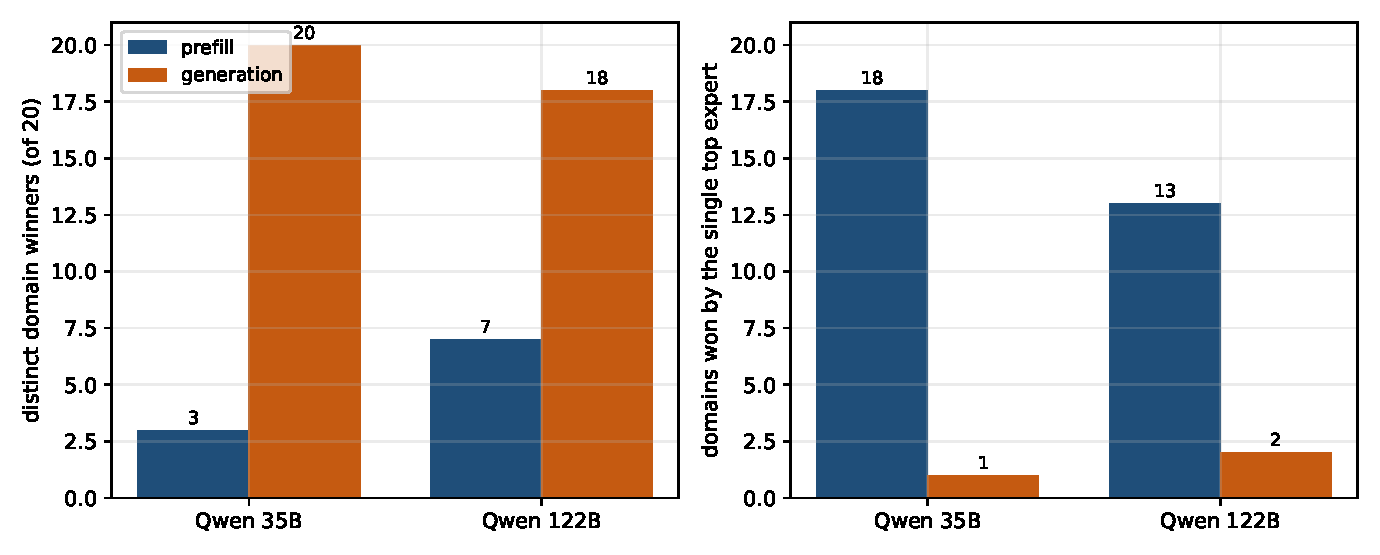
\includegraphics[width=0.9\textwidth]{figures/fig1_distinct_winners.pdf}
\caption{Left: number of distinct experts among the 20 domain winners.
Right: number of domains won by the single most frequent winner. In both
models the prefill winners collapse onto a generalist and the generation
winners spread across the domains. $n=60$ prompts per model (20 domains
$\times$ 3).}
\label{fig:winners}
\end{figure*}

\begin{table*}[t]
\centering
\small
\begin{tabular}{llrrrr}
\toprule
Model & Regime & Distinct winners & Max wins & Herfindahl & Norm.\ entropy \\
\midrule
Qwen 35B  & prefill    & 3  & 18 & 0.815 & 0.13 \\
Qwen 35B  & generation & 20 & 1  & 0.050 & 1.00 \\
Qwen 122B & prefill    & 7  & 13 & 0.445 & 0.42 \\
Qwen 122B & generation & 18 & 2  & 0.060 & 0.95 \\
\bottomrule
\end{tabular}
\caption{Concentration of the 20-domain winner list, by model and regime.
Distinct winners and max wins are counts out of 20 domains; Herfindahl and
normalized entropy are computed on the distribution of domains won per expert
(Section~\ref{sec:methods}). Each row summarizes one domain-winner table from
the source archive ($n=60$ prompts per model, 3 per domain).}
\label{tab:conc}
\end{table*}


\paragraph{Probe.}
The prompt suite contains 60 short questions covering 20 academic domains
(archaeology, biology, chemistry, comparative religion, computer science,
cybersecurity, economics, environmental science, history, law, linguistics,
mathematics, medicine, neuroscience, philosophy, physics, political science,
psychology, software engineering, statistics), three per domain. Each is a
plain, domain-typical prompt, for example a request to contrast two core
concepts in the field.

\paragraph{Models.}
We use two MoE checkpoints from the Qwen3.5 lineage \citep{yang2025qwen3},
both 8-bit quantized community fine-tunes (HauhauCS variants): a
35B-parameter model with about 3B parameters active per token
(Qwen3.5-35B-A3B) and a 122B-parameter model with about 10B active
(Qwen3.5-122B-A10B). Both route each token to the top 8 of 256 experts per
MoE layer. The two models have different layer counts and internal layouts,
so their expert indices are unrelated: an expert numbered 114 in one has
nothing to do with expert 114 in the other. Decoding is greedy with no
reasoning trace. Generation is capped at 2,048 to 2,056 new tokens; we return
to the cap in Section~\ref{sec:limits}.

\paragraph{Routing reconstruction.}
For each token we take the router's pre-softmax logits over all 256 experts,
apply a softmax, keep the top 8, and renormalize so the eight weights sum to
one. For an expert $e$ on a fixed set of tokens (one regime of one prompt at
one layer) we form three reductions of these weights: $S_e$, the fraction of
tokens on which $e$ is selected; $Q_e$, its mean weight on tokens where it is
selected; and $W_e$, its mean weight over all tokens (zero where unselected).
Because all three reduce the same weights, $W_e=S_eQ_e$ holds exactly on any
single token set; we use this as a bookkeeping check that the selection mask,
conditional mean, and marginal mean are mutually consistent
($\max_e|W_e-S_eQ_e|\le5.6\times10^{-17}$ across all capture cells). The
identity holds per token set only; the tabulated per-domain $S$ and $Q$ in
the accompanying data are separate means whose product differs from the
tabulated $W$ by the across-prompt covariance.
Domain winners are ranked by $W$, the mean routed weight per token.

\paragraph{The two regimes and the domain winner.}
For each prompt we partition its token positions into the prefill block (the
prompt tokens) and the generation block (the tokens the model produced). All
routing statistics are computed within one block, never pooled across them.
For each domain we form the per-domain mean of $W_e$ over the domain's three
prompts and all MoE layers and call the highest-$W$ expert the \emph{domain
winner}. This yields, per model and per regime, a list of 20 domain winners;
the analysis concerns how the two lists differ. We call the expert that wins
the most domains in a list the \emph{generalist}.

\paragraph{Concentration of a winner list.}
A list of 20 winners is summarized by its \emph{distinct count} (how many
different experts appear), its \emph{max wins} (domains taken by the single
most frequent winner), the Herfindahl index $\sum_i p_i^2$, and the normalized
Shannon entropy $H=-\sum_i p_i\log_2 p_i/\log_2 20$, where $p_i$ is the
fraction of domains won by expert $i$; $H$ runs from 0 (one expert wins every
domain) to 1 (every domain has its own winner). These are deterministic
summaries of the winner lists.

\paragraph{Token-balanced control.}
To separate the regime from token count, three prompts were each packed with
twenty domain questions and padded to exactly 446 prompt tokens, and each was
allowed 2,048 generated tokens, so the prefill and generation blocks are
matched in scale and per-chunk comparisons use identical token budgets. For
each chunk we report the Jaccard index (intersection over union) between the
prefill and generation top-expert sets, ranked by $W$ and by $S$, and the mean
per-token routing entropy of each regime.

\section{Results}
\label{sec:results}

\begin{figure}[t]
\centering
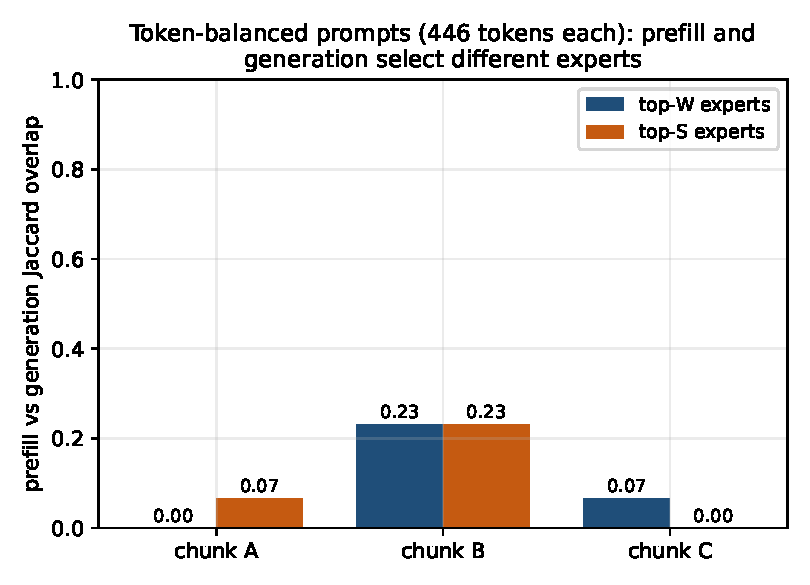
\includegraphics[width=\columnwidth]{figures/fig3_token_balanced.pdf}
\caption{Token-balanced control (35B model, three packed prompts of 446
prompt tokens and 2,048 generated tokens each). Jaccard overlap between the
prefill and generation top-expert sets, ranked by routed weight and by
selection rate. With token counts matched, the two regimes select largely
disjoint experts.}
\label{fig:balanced}
\end{figure}


\subsection{Over prefill one generalist wins almost every domain}

In the 35B model the prefill winner list is dominated by a single expert that
takes 18 of the 20 domains; only chemistry and linguistics have their own
prefill winners. The same expert is the top expert overall on the prefill
block. The list has 3 distinct experts and normalized entropy 0.13
(Table~\ref{tab:conc}). Read literally, prefill routing assigns one
high-frequency default to nearly every subject. In the 122B model a different
generalist wins 13 of 20 domains, with a second expert taking 2 more, for 7
distinct winners and entropy 0.42: less extreme, and still strongly
concentrated.

\subsection{Over generation the winners disperse to distinct per-domain experts}

The generation winner list for the same 35B model and prompts diverges
sharply. All 20 domains are won by 20 distinct experts; no expert wins more
than one domain, and normalized entropy rises from 0.13 to 1.00. The
generalist that won 18 domains during prefill wins exactly one during
generation (political science). Domain-specific experts surface in its place:
the philosophy generation winner, for instance, held only rank 5 within
philosophy during prefill ($W=0.0188$ over generation against a mid-pack
prefill weight) and wins no other domain. The 122B model shows the same
dispersion, to 18 distinct winners across the 20 domains (two experts win two
domains each), entropy 0.95, and its global top experts also change identity
between regimes. The generalist's reach falls from 18 to 1 domains in the 35B
model and from 13 to 2 in the 122B model (Figure~\ref{fig:winners}).

The dispersion holds regardless of where the generated text is cut. These
checkpoints render the end-of-turn marker as literal text and continue into
synthetic follow-up turns until the token cap. Trimming the generation block at that marker or leaving it
untrimmed produces the same 20 distinct domain winners in the 35B model. The
structure sits in the answer content.

\subsection{The shift persists at matched token count}

The dispersion is a regime effect. Prefill and generation differ in length
(a prompt is tens of tokens and an answer hundreds), so the token-balanced
control asks whether longer token sets alone could disperse the top experts.
With prefill and generation matched at 446 and 2,048 tokens per chunk, the
Jaccard overlap between the top-expert sets of the two regimes is 0.00, 0.23,
and 0.07 across the three chunks by routed weight and 0.07, 0.23, and 0.00 by
selection rate (Figure~\ref{fig:balanced}): the experts that dominate
generation are mostly disjoint from those that dominate prefill at matched
token count. Per-token routing entropy is almost unchanged between regimes
(0.958 prefill, 0.953 generation), so generation spreads each token over a
similar number of experts and routes it to different ones. The regime moves
the winners while length is held fixed.

\subsection{The pattern reproduces with unrelated expert indices}

The 122B model is an independent replication in the sense that matters: its
expert indices are unrelated to the 35B model's, its generalist is a
different expert, and its prefill leaders and generation leaders are
different sets of indices, yet the prefill-concentrated, generation-dispersed
shape carries over (Table~\ref{tab:conc}). The two models also show that an
expert's role can move between regimes within a model and that indices are
model-specific: in the 122B model the expert leading philosophy generation is mid-pack
in philosophy prefill, and the index that wins philosophy generation in the
35B model has, in the 122B model, its only strong footprint in computer
science. We read these as cautions against naming experts from any single
regime or carrying an index across models.

\section{Discussion}
\label{sec:discussion}

\paragraph{What the measurement establishes.}
In these models routing over prompt positions is dominated by a few
high-frequency experts and carries little domain signal, while routing over
generated positions resolves into distinct per-domain leaders. Domain
specialization, to the extent the router expresses it, is a property of the
generation regime. A deflationary reading would credit the dispersion to
generation routing more diffusely in general; the two entropies measured
together in the token-balanced control tell against it. Per-token routing
entropy holds nearly steady across regimes (0.958 against 0.953) while the
winner-distribution entropy moves from 0.13 to 1.00 in the 35B model and from
0.42 to 0.95 in the 122B model. The per-token spread stays put; the identity
of each domain's leading expert changes. That relabeling is the specialization
signal.

\paragraph{A candidate cause.}
A plausible reading gives the negative results a principled cause: reading a
short prompt is a fairly generic operation (tokenizing, parsing, building
context) for which the router falls back on broadly useful experts, and
domain-specific computation is recruited once the model commits to producing
domain-specific content token by token. On that reading supplied-text routing
misses domain structure because it observes the model only during the regime
that has yet to recruit the domain machinery. This is a hypothesis about the
cause; the data locate the effect.

\paragraph{Implication for how specialization is measured and read.}
An analysis that characterizes expert-topic structure from prefill routing,
or from routing pooled over a sequence without separating the regimes, sees
the concentrated prefill picture and understates specialization. The same
probe read over generation recovers per-domain structure. Two consequences
follow. First, negative results obtained over supplied text, including the
canonical Mixtral analysis \citep{jiang2024mixtral}, report the prefill regime
and are silent about generation; the demonstrated claim covers the Qwen3.5
lineage, and the reading of any particular prior result as understated is an
inference from the measurement convention, since we re-measure none of them. Second, routing analyses that ask what experts specialize in
should measure the two regimes separately and read specialization from
generation; expert-identification methods, benchmark suites for
specialization, and expert-naming pipelines that operate on supplied text
inherit the prefill picture by construction. The result leaves open what the generation-regime experts encode, and
analyses of prefill routing for their own sake are unaffected by it.

\section{Limitations}
\label{sec:limits}

Both checkpoints are 8-bit quantized community fine-tunes of Qwen3.5 MoE
models; the pattern reproduces across two sizes with non-corresponding
indices, which supports the method-level reading, but the demonstrated claim
covers this lineage. Generated blocks are long and frequently reach the cap
(in the 122B run 49 of 60 cells hit 2,048 tokens, mean generated length about
1,868), and every cell eventually spills into chat-template continuation;
trimming at the spill boundary leaves the 35B winner list unchanged, which
argues against a spill artifact, while generation budgets vary per
prompt. The domain winner is a coarse statistic that treats a domain with two
near-tied leaders and a domain with one dominant expert alike, and with three
prompts per domain it is the least reliable layer of the analysis; the claims
rest on the aggregate concentration contrasts alone; no single domain's
assignment is load-bearing. The concentration summaries are descriptive: no randomization
null is attached to the 18-versus-20 and 13-versus-18 contrasts, although
their size leaves little room for chance dispersion.

\section{Conclusion}
\label{sec:conc}

Two MoE language models route prompt tokens and generated tokens to different
experts, and the difference is structured: over the prompt-reading regime a
single generic expert wins almost every domain, and over the generation regime
the domains acquire distinct leading experts. The shift is large, survives
matching the regimes in token count, and reproduces across two model sizes
with unrelated expert indices. Expert specialization measured over
supplied text, the regime that is cheap and deterministic to capture, is
therefore understated by construction, and the negative results built on such
measurements are silent about the regime in which specialization is
expressed. Analyses that ask what an MoE's experts specialize in should
separate the two regimes and read specialization from generation.

\section*{Data and Code Availability}
\addcontentsline{toc}{section}{Data and Code Availability}

The data supporting this paper accompany it in the \texttt{data/} directory,
organized as three runs: the 35B 60-prompt primary probe, the 35B
token-balanced three-chunk control, and the 122B replication (prefill and
generation captures). Each run folder contains the per-domain winner tables
from which every number in the paper is taken; \texttt{data/README.md} maps
each run to the claims it supports, and \texttt{SOURCES.md} gives a
claim-by-claim source index. The two figures and the concentration summaries
in Table~\ref{tab:conc} are reproduced from the winner lists by
\texttt{make\_figures.py}, which re-runs no model. Raw router tensors
(\texttt{.npz}) are included as non-load-bearing provenance. Two provenance
choices are stated plainly: the 122B analysis was framed in its source notes
around locating an analog of one particular expert, and we set that framing
aside and report only the regime-dependent concentration the same tables
support; and we use the reconstructed, log-derived routing tables in place of
earlier hand-summarized figures. No new model training was performed.

\section*{AI Collaboration Statement}
\addcontentsline{toc}{section}{AI Collaboration Statement}

Generative AI (Anthropic's Claude) was used as a tool in preparing this
manuscript: to assist with drafting and revising prose, organizing the
manuscript, and locating and formatting the bibliography. All experiments,
captures, and numerical results are the author's; every reported value was
traced to a source capture (see \texttt{SOURCES.md}), and every reference was
verified by the author against its authoritative record. No AI system is an
author. The author reviewed the entire text and takes full responsibility for
its content.

\section*{Funding and Competing Interests}
\addcontentsline{toc}{section}{Funding and Competing Interests}

This work received no external funding. The author declares no competing
interests. The models studied are third-party fine-tunes used as-is for
measurement; the author has no affiliation with their creators.

\bibliographystyle{plainnat}
\bibliography{refs}

\end{document}
